
\chapter{Nonlinear Problems}\label{chap9}

\subsubsection{\bf Introduction.} We\pageoriginale consider here
problems of the following type:

Find $u\varepsilon C$ such that
\begin{equation}\label{chap9:eq9.1}
J(u)\leq J(v)\quad\text{for all } v\;\varepsilon \;V,
\end{equation}
where $C$ is a closed, convex subset of a Banach space $V$ and
$J:V\to\mathbb{R}$ is a convex, lower semi-continuous $(l.s.c.)$ function.

We denote by $(\cdotp,\cdotp)$ the duality pairing $V'-V$ and
$\parallel \cdotp\parallel$ the norm in $V$. We write
\eqref{chap9:eq9.1} in the form:

Find $u\varepsilon C$ such that 
\begin{equation}\label{chap9:eq9.2}
J(u)=\underset{v\varepsilon C}{\Inf}\;J(v).
\end{equation}

The existence and uniqueness of the solutions of \eqref{chap9:eq9.2}
is given by 

\setcounter{THM}{0}
\begin{THM}\label{chap9:THM1}
Assume that $J$ is coercive on $C$, that is 
\begin{equation}\label{chap9:eq9.3}
J(v)\to\infty\quad\text{if}\quad\parallel v\parallel\to\infty, v
\;\varepsilon \;C.
\end{equation}
Then problem \eqref{chap9:eq9.2} has atleast one solution provided
that $V$ is reflexive.

If $J$ is strictly convex, then \eqref{chap9:eq9.2} has almost one solution.
\end{THM}

The proof of theorem \ref{chap9:THM1} can be found in EMELAND-TEMAN \cite{key15}.

\setcounter{exercise}{0}
\begin{exercise}\label{chap9:exr1}
If\pageoriginale $J$ is Gateaux-differentiable, then $u$ is a solution
of \eqref{chap9:eq9.2} $\Iff$
$$
(J'(u),v-u)\geq 0\quad\text{for all } v\;\varepsilon \;C.
$$
If $C$ is affine linear, \eqref{chap9:eq9.1} implies 
$$
(J'(u),v-u)=0\;\forall \;v\;\varepsilon\;C.
$$
\end{exercise}

\medskip
\noindent{\textbf{Approximation.}}

 Let $V_h$ be a finite-dimensional
subspace of $V$ and $C_h$ a closed, convex subset of $V_h$. Then the
approximate problem corresponding to \eqref{chap9:eq9.2} is:

Find $u_h\;\varepsilon\;C_h$ such that 
\begin{equation}\label{chap9:eq9.4}
J(u_h)=\underset{v_h\varepsilon C_h}{\Inf}\;J(v_h).
\end{equation}

We assume that $J$ is strictly convex and coercive. Moreover, we
assume that $C_h$ approximates $C$.
\begin{equation}
\left.
\begin{aligned}
&\text{For all } v\;\varepsilon \;C\quad\text{there exists}\quad
v_h \;\varepsilon \;C_h\\
&\text{such that}\quad v_h\to v\quad\text{(strongly) as}\quad h\to
0;\\ \label{chap9:eq9.5}
\end{aligned}
\right\}
\end{equation}
\begin{equation}
\left.
\begin{aligned}
&\text{If}\quad w_h\rightharpoonup w\;\varepsilon \;V\quad\text{as}
\quad h\to 0\quad\text{and}\quad w_h\;\varepsilon \;C_h\\
&\text{then}\quad w\;\varepsilon \;C. \label{chap9:eq9.6}
\end{aligned}
\right\}
\end{equation}
Then one can easily prove that the solution $u_h$ of
\eqref{chap9:eq9.4} converges weakly to $u$, the solution of
\eqref{chap9:eq9.2}.

Note that \eqref{chap9:eq9.5} implies that $C_h$ has to be
sufficiently big and \eqref{chap9:eq9.6} demands $C_h$ to be
sufficiently small.

To\pageoriginale get strong convergence of $u_h$ to $u$, one needs
some strong monotonicity; there exists $\alpha,\gamma >0$ such that 
\begin{equation}\label{chap9:eq9.7}
(J'(u)-J'(v),u-v)\geq\alpha\parallel u-v\parallel^\gamma,\forall \,u,
\;v \;\varepsilon \;C
\end{equation}

\begin{case}\label{chap9:case1}
We obtain an error estimate when $C_h=C\cap V_h$. From Exercise
\ref{chap9:exr1}, we have 
\begin{align}
(J'(u),v-u)\geq 0\;\forall \;v\;\varepsilon \;C, \label{chap9:eq9.8}\\
(J'(u_h),\;v_h-u_h)\geq 0\; \; \forall \;v_h\;\varepsilon
\;C_h. \label{chap9:eq9.9} 
\end{align}

As $C_h=C\cap V_h$, choosing $v=u_h$ in \eqref{chap9:eq9.8} and adding
to \eqref{chap9:eq9.9}, we get 
$$
(J'(u)-J'(u_h),u_h-u)+(J'(u_h),\;v_h-u)\geq 0.
$$
Therefore (assuming $J$ to be continuously differentiable)
$$
\alpha\parallel u_h-u\parallel^\gamma\leq(J'(u_h),v_h-u)\leq
c\parallel v_h-u\parallel,
$$
since $u_h$ is bounded. Finally,
\begin{equation}\label{chap9:eq9.10}
\parallel u_h-u\parallel\leq c\underset{v_h\varepsilon C_h}{\Inf}
\parallel v_h-u\parallel^{1/\gamma},
\end{equation}
provided $J'$ is weakly continuous.

Note that 
$$
\underset{v_h\varepsilon C_h}{\Inf}\parallel v_h-u\parallel
$$
measures how good is the approximation $C_h$ to $C$. Note also that,
as $u_h$ is bounded, it is enough if \eqref{chap9:eq9.7} holds on
bounded subsets of $C$. 
\end{case}

\begin{exercise}\label{chap9:exr2}
Let\pageoriginale $\phi:V\to\mathbb{R}$ be Lipschitz but not
differentiable. Then 
$$
J(u)=\underset{v\varepsilon C}{\Inf}[J(v)+\phi(v)]
$$
is equivalent to 
$$
(J'(u),v-u)+\phi(v)-\phi(u)\geq 0\; \; \forall \;v\;\varepsilon \;C.
$$
Derive an error estimate similar to \eqref{chap9:eq9.10}.
\end{exercise}

\begin{case}\label{chap9:case2}
When $C$ is of the form
\begin{equation}\label{chap9:eq9.11}
C=\{v\;\varepsilon \;V:b(v,\mu)=(\phi,\mu)\; \; \forall \;\mu
\;\varepsilon \;M\},
\end{equation}
where $M$ is a Hilbert space, $b(\cdotp,\cdotp)$ is a continuous,
bilinear form on $V\times M$ and $\phi\varepsilon M$ satisfying
Brezzi's condition (See Chapter \ref{chap7}), Problem
\eqref{chap9:eq9.1} is equivalent to:

Find $\{u,\lambda\}\;\varepsilon \;V\times M$ such that
\begin{equation}\label{chap9:eq9.12}
<J'(u),v>+b(v,\lambda)=0\; \; \forall \;v \;\varepsilon \;V,
\end{equation}
\begin{equation}\label{chap9:eq9.13}
b(u,\mu)=(\phi,\mu)\; \; \forall \;\mu \;\varepsilon \;M.
\end{equation}

We notice that \eqref{chap9:eq9.11} is affine linear and from Exercise
\ref{chap9:exr1} we obtain that \eqref{chap9:eq9.1} is equivalent to
\begin{equation}\label{chap9:eq9.14}
(J'(u),v-u)=0\; \; \forall \;v \;\varepsilon \;C.
\end{equation}
Let $B:V\to M$ be defined by 
$$
(Bv,\mu)=b(v,\mu)\; \; \forall \;v \;\varepsilon \;V, \;\mu \;\varepsilon
\;M.
$$
Clearly\pageoriginale $C=v+\Ker B$, where $v\varepsilon C$. This
together with \eqref{chap9:eq9.14} implies
$$
J'(u)\;\varepsilon \;(\Ker B)^\bot=\Iim B^*,
$$
which is closed from Brezzi's condition. Hence there exists $\lambda
\varepsilon M$ such that
$$
J'(u)=-B^*\lambda.
$$
Thus
$$
(J'(u), \;v)+b(v,\lambda)=0\; \; \forall \;v\;\varepsilon \;V.
$$
$u\varepsilon C$ implies $b(u,\mu)=(\phi,\mu)\forall \mu\varepsilon
M$.

So we have proved that \eqref{chap9:eq9.1} implies
\eqref{chap9:eq9.12} and \eqref{chap9:eq9.13}.

If \eqref{chap9:eq9.12} and \eqref{chap9:eq9.13} hold, then
$u\varepsilon C$ and 
$$
(J'(u),u)=-b(u,\lambda)=-b(v,\lambda)\; \; \forall \;v\;\varepsilon \;C
$$
Hence $ \langle J'(u),v-u \rangle =0 \; \; \forall v\varepsilon C$, which is equivalent to \eqref{chap9:eq9.1}. 

Thus we proved the equivalence of \eqref{chap9:eq9.1} and
\eqref{chap9:eq9.12} \eqref{chap9:eq9.13}.

$A$ natural approximation $C_h$ to $C$ will be 
$$
C_h=\{v\;\varepsilon \;V:b(v,\mu_h)=(\phi,\mu_h)\; \; \forall \;\mu_h
\;\varepsilon \;M_h\},
$$
where $M_h$ approximates $M$. In this case 
$$
C_h\nsubset C.
$$
\end{case}

\setcounter{exam}{0}
\begin{exam}\label{chap9:exm1}
{Nonlinear Dirichlet Problem.}\pageoriginale 
\begin{align*}
&V=W^{1,p}(\Omega), C=V\\
&J(v)=\frac{1}{p}\int\limits_\Omega|\nabla v|^p\,dx-\int\limits_\Omega
  fv \,dx,
\end{align*}
where
$$
f\;\varepsilon \;L^q, \;1/p+1/q=1
$$
For $1<p<\infty, W^{1.p}(\Omega)$ is reflexive and $J(v)\to\infty$ as
$\parallel v\parallel \to\infty$. One has 
$$
(J'(u),v)=\int\limits_\Omega |\nabla u|^{p-2}\nabla u.\nabla v\;\,dx-
\int\limits_\Omega fv\,dx,
$$
and some strong monotonicity results of the type \eqref{chap9:eq9.7}
are proved in GLOWINSKI-MARROCCO \cite{key19}.
\end{exam}
 
\begin{exam}\label{chap9:exm2}
{The Obstacle Problem.}
\begin{align*}
V &= H_\circ^1(\Omega),\\
C &=\{v\;\varepsilon \;H_\circ^1(\Omega):v\geq 0 \;\Ae\quad
\text{on}\quad \Omega\},\\
J(v) &= \frac{1}{2}\int\limits_\Omega|\nabla v|^2\,dx-
\int\limits_\Omega fv \,dx.
\end{align*}

Existence and uniqueness of the solution of the minimization problem
are straightforward.

Let $V_h$ be the standard Lagrange finite element space of degree 1
and $C_h=C\cap V_h$. One has \eqref{chap9:eq9.10} with $\gamma=2$;
therefore it seems that one gets 
$$
\parallel u-u_h\parallel=0(\sqrt{h})
$$\pageoriginale
since the interpolate $\pi_h u\varepsilon C_h$ as long as
$u\varepsilon C$. However, one has 
\begin{gather*}
(J'(u_h),v_h-u)=(J'(u),v_h-u)+(J'(u_h)-J'(u),v_h-u)\\
\leq(-\Delta u-f,v_h-u)+\frac{M\varepsilon}{2}\parallel u_h-u
\parallel_1^2+ \frac{M}{2\varepsilon}\parallel v_h-u\parallel_1^2. 
\end{gather*}
Hence
$$
\parallel u-u_h\parallel_1^2\leq c\left(\parallel v_h-u\parallel_0^2
+\parallel v_h-u\parallel_1^2\right)
$$
Therefore
$$
\parallel u-u_h\parallel_1=0(h).
$$
\end{exam}

\begin{exam}\label{chap9:exm3}
{Elasto - Plastic Torsion.} $J$ and $V$ as is Example
\ref{chap9:exm2}, 
$$
C=\{v\;\varepsilon \;H_\circ^1(\Omega):|\nabla v|\leq 1\Ae
\quad\text{on}\quad\Omega\},
$$
$V_h$ same as in Example \ref{chap9:exm2} and $C_h=C\cap V_h$. 

In this case the interpolate $\pi_hu$ is not in $C_h$ whereas $u$ is
in $C$. One gets $0(h^{1/2-\varepsilon})$.
\end{exam}

\begin{exam}\label{chap9:exm4}
{The Flow of a Bingham Fluid in a Cylindrical Pipe.} This is a
particular case of Exercise \ref{chap9:exr2} with $J,V$ as above and 
$$
\phi(v)=\int\limits_\Omega |\nabla v|\,dx.
$$
\end{exam}

\setcounter{section}{1}
\section{Generalization}\label{chap9:sec2} 
Note that $J':V\to V'$ satisfies 
$$
(J'(u)-J'(v),u-v)\geq 0\; \; \forall \;u,v \;\varepsilon \;V.
$$\pageoriginale

An operator $A:V\to V'$ is said to be \emph{monotone} if 
\begin{equation}\label{chap9:eq9.15}
(Au-Av, u-v)\geq 0\; \; \forall \;u, \;v \;\varepsilon \;V.
\end{equation}

$A$ is \emph{bounded} if $A$ maps bounded sets of $V$ into bounded
sets of $V'$. 

$A$ is \emph{hemi-continuous} if 
\begin{equation}\label{chap9:eq9.16}
\lim\limits_{\lambda\to 0}\;(A(u+\lambda w),v)=(A(u),v)\; \; \forall \;u,
v, w\;\varepsilon \;V.
\end{equation}

$A$ is \emph{coercive} if 
\begin{equation}\label{chap9:eq9.17}
\frac{(A(v),v)}{\parallel v\parallel}\to \infty \;\text{if}\;
\parallel v\parallel \to \infty \;\text{for}\; v\;\varepsilon \;C.
\end{equation}

We have 
\begin{THM}\label{chap9:THM2}
If $A$ is a monotone, bounded hemi continuous and coercive operator
then the problem:

Find $u\varepsilon C$ such that 
\begin{equation}\label{chap9:eq9.18}
(A(u),v-u)\geq 0\; \; \forall \;v \;\varepsilon \;C
\end{equation}
has atleast one solution.
\end{THM}

For a proof of this Theorem see LIONS \cite{key28}. The problem
\eqref{chap9:eq9.18} has at most one solution if $A$ is \emph{strongly
  monotone}, \ie there exists $\alpha,\gamma >0$ such that
\begin{equation}\label{chap9:eq9.19}
\alpha\parallel u-v\parallel^\gamma\leq(A(u)-A(v),u-v)\; \; \forall \;u,v
\;\varepsilon \;C
\end{equation}
The error analysis can be carried out in the same way. 

\section{Contractive Operators.}\label{chap9:sec3}
Let\pageoriginale $T:C\to C$ be a mapping, where $C$ is a closed,
convex subset of a Hilbert space $H$. The scalar product in $H$ is
denoted by $(\cdotp,\cdotp)$. 

We call $T$ \emph{contractive} $\Iff$ 
\begin{equation}\label{chap9:eq9.20}
\parallel Tx-Ty\parallel \leq \parallel x-y\parallel, \; \; \forall \;x,
\;y \; \varepsilon \;C.
\end{equation}
$T$ is \emph{strictly contractive} $\Iff$ there exists a $\theta$ with
$0<\theta <1$ such that 
\begin{equation}\label{chap9:eq9.21}
\parallel Tx-Ty\parallel \leq \theta\parallel x-y\parallel \; \; \forall
\;x, \;y \;\varepsilon \; C.
\end{equation}
We say that $T$ is \emph{firmly contractive} $\Iff$ (\cf
BROWDER-PETRYSHN \cite{key8})
\begin{equation}\label{chap9:eq9.22}
\parallel Tx-Ty\parallel^2 \leq (Tx-Ty, x-y)\; \; \forall \;x, \;y
\;\varepsilon \;C
\end{equation}
$T$ is \emph{quasi firmly contractive} $\Iff$ there exists a $\theta,
0<\theta <1$ such that 
\begin{equation}\label{chap9:eq9.23}
\parallel Tx-Ty\parallel^2 \leq \theta(Tx-Ty, x-y)+(1-\theta)\parallel
x-y\parallel^2 
\end{equation}

Note that \eqref{chap9:eq9.22}$\Rightarrow$ \eqref{chap9:eq9.23}
$\Rightarrow$ \eqref{chap9:eq9.20} and \eqref{chap9:eq9.21}$\Rightarrow$
\eqref{chap9:eq9.20}. 

\medskip
\noindent{\textbf{Geometrical Interpretation of the Above  Definitions}}
 Let $y\varepsilon C$ be a fixed point of $T$, \ie
$Ty=y$. If $T$ is contractive and $x\varepsilon C$ then
$Tx$ lies in the closed ball with $y$ as centre and
$\parallel y-x\parallel$ as radius. If $T$ is strictly
contractive, then $Tx$ lies in the open ball with $y$ as centre and
$\parallel y-x\parallel$ as radius, for all $x\varepsilon C$. If $T$
is firmly contractive then from \eqref{chap9:eq9.22} we obtain 
$$
(Tx-y,x-Tx)\geq 0\; \; \forall \;x \;\varepsilon \;C.
$$\pageoriginale
This means that the angle between $y-Tx$ and $x-Tx$ is obtuse.
\begin{figure}[H]
\centering
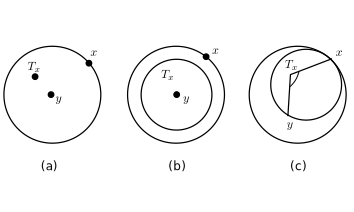
\includegraphics{figure/addfig9.1.eps}
\caption{}\label{fig9.1}
\end{figure}

Note that if $T_1$ and $T_2$ are contractive then $T=T_1 T_2$ is
contractive and $T$ is strictly contractive if any one of $T_1$ and
$T_2$ is. However, $T_1, T_2$ firmly (or quasi-firmly) contractive
implies \emph{only} $T=T_1 T_2$ is \emph{contractive}.

\noindent {\bf Fixed Points.} We recall that $x$ is a fixed point of $T \Iff
Tx=x$. Let $F(T)$ denote the set of all fixed points of $T$. If $T$ is
strictly contractive then $T$ has a unique fixed point and $F(T)$ is
singleton. We have 

\begin{THM}\label{chap9:THM3}
If $T$ is contractive, then $F(T)$ is closed and convex.
\end{THM}

\begin{proof}
Let $x_n\varepsilon F(T), x_n\to x$. Then 
$$
\parallel x_n-Tx\parallel \leq \parallel x_n-x\parallel
$$
Taking the limit as $n\to\infty$ we get $\parallel x-Tx\parallel=0,
\ie x\varepsilon F(T)$. Hence\pageoriginale $F(T)$ is closed.

Let $x, y \varepsilon F(T)$ and $u=\theta x+(1-\theta)$ where
$0<\theta <1$. We have 
\begin{align}
&\parallel x-Tu\parallel \leq\parallel x-u\parallel=(1-\theta)
\parallel x-y\parallel, \label{chap9:eq9.24}\\
&\parallel y-Tu\parallel \leq\parallel y-u\parallel=\theta \parallel
x-y\parallel, \label{chap9:eq9.25}\\
&\parallel x-y\parallel\leq\parallel x-Tu\parallel +\parallel
y-Tu\parallel \leq\parallel x-y\parallel, \label{chap9:eq9.26}
\end{align}
Since $H$ is strictly convex, we obtain using \eqref{chap9:eq9.24} and
\eqref{chap9:eq9.25}, 
\begin{align}
&x-Tu=c(y-Tu)\label{chap9:eq9.27}\\
&\parallel x-Tu\parallel^2=c(y-Tu,x-Tu), \label{chap9:eq9.28}
\end{align}
$$
\parallel x-y\parallel^2=\parallel x-Tu\parallel^2+\parallel y-Tu
\parallel^2+2\parallel x-Tu\parallel \;\parallel y-Tu\parallel,
$$
by \eqref{chap9:eq9.26},
\begin{align*}
\parallel x-y\parallel^2 &= \parallel x-Tu+Tu-y\parallel^2\\
&= \parallel x-Tu\parallel^2 +\parallel Tu-y\parallel^2 +2(x-Tu, Tu-y) 
\end{align*}
So
\begin{equation}\label{chap9:eq9.29}
(x-Tu, Tu-y)=\parallel x-Tu\parallel \; \parallel y-Tu\parallel >0.
\end{equation}
From \eqref{chap9:eq9.28} and \eqref{chap9:eq9.29} we obtain $c<0$.

Equations \eqref{chap9:eq9.26} and \eqref{chap9:eq9.27} imply
$$
\parallel y-Tu\parallel =\frac{1}{1+|c|}\;\parallel x-y\parallel.
$$
This with \eqref{chap9:eq9.25} gives $|c|\geq
(1-\theta)\theta^{-1}$. Similarly using \eqref{chap9:eq9.24},
\eqref{chap9:eq9.26} and \eqref{chap9:eq9.27} we obtain $|c|\leq
(1-\theta)\theta^{-1}$. Thus 
$$
|c|=(1-\theta)\;\theta^{-1}.
$$\pageoriginale
Hence
$$
\theta(x-Tu)=-(1-\theta)(y-Tu).
$$
Therefore
$$
Tu=\theta x+(1-\theta)y=u,
$$
that is 
$$
u\;\varepsilon \;F(T).
$$
\end{proof}

\setcounter{REM}{0}
\begin{REM}\label{chap9:rem1}
Theorem \ref{chap9:THM3} can be proved geometrically.

Let $u=\theta x+(1-\theta)y$, $x,y\varepsilon F$. Since $x\varepsilon
F(T)$ and $T$ is contractive $Tu$ lies in the closed ball $C_x$ with
$x$ as centre and $\parallel x-u\parallel$ as radius. Similarly $Tu$
lies in the closed ball $C_y$ with $y$ as centre and $\parallel
y-u\parallel$ as radius. But $C_x\cap C_y=u$. Hence $Tu=u$. Thus
$u\varepsilon F(T)$ and $F(T)$ is convex. 
\end{REM}
\begin{figure}[H]
\centering
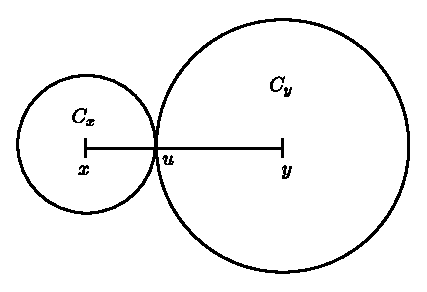
\includegraphics{figure/fig9.2.eps}
\caption{}\label{fig9.2}
\end{figure}

If $C$ is bounded and $T$ is contractive, then 
$$
F(T)\neq \phi.
$$

In\pageoriginale the following we assume $F(T)\neq\phi$ and study the
convergence of the iterative method
$$
x^{n+1}=Tx^n.
$$
which is known to be strongly convergent to the unique fixed point of
$T$ if $T$ is strictly contractive. One has 

\begin{THM}\label{chap9:THM4}
If $T$ is firmly contractive and $F(T)\neq\phi$ then 
$$
x^n\rightharpoonup\xi \;\varepsilon \;F(T)\quad\text{as}\quad
n\to\infty
$$
$\ie x^n$ converges weakly to a fixed point.
\end{THM}

\begin{proof}
Let $y\varepsilon F(T)$. We have 
$$
\parallel x^{n+1}-y\parallel^2\leq(x^{n+1}-y,x^n-y)
$$
But 
\begin{align*}
\frac{1}{2}\parallel x^{n+1}-x^n\parallel^2 &=\frac{1}{2}\parallel
x^{n+1}-y\parallel^2+\frac{1}{2}\parallel x^n-y\parallel^2-(x^{n+1}
-y, x^n-y)\\
&\leq \frac{1}{2}\parallel x^n-y\parallel^2-\frac{1}{2}\parallel
x^{n+1}-y\parallel^2.
\end{align*}
Therefore
\begin{align*}
&\parallel x^{n+1}-y\parallel^2+\parallel x^{n+1}-x^n\parallel^2 \leq
\parallel x^n-y\parallel^2,\\
&\parallel x^{N+1}-y\parallel^2+\sum\limits_{n=0}^N\parallel x^{n+1}-
x^n\parallel^2 \leq\parallel x^\circ -y\parallel^2,
\end{align*}
which proves that $\parallel x^{n+1}-x^n\parallel\to 0$ and $\{x^n\}$
is a bounded sequence. Let $x^{n'}\rightharpoonup x$ be a weakly
convergent subsequence.

Since\pageoriginale
$$
(Tx-Ty, \;Tx-Ty+y-x)\leq 0
$$
choosing $y=x^{n'-1}$ we obtain 
$$
\left(Tx-x^{n'},\; Tx-x^{n'}+x^{n'-1}-x\right)\leq 0
$$
As $n' \to \infty$, we get
$$
(Tx-x,\;Tx-x)\leq 0,
$$
and hence $x\varepsilon F(T)$. 

As $\parallel x^n-y\parallel^2$ is a decreasing sequence for any
$y\varepsilon F(T)$ it converges to some number $P(y)$, and we
conclude from the following Lemma that the whole sequence $x^n$ converges. 
\end{proof}

\setcounter{opal lem}{4}
\begin{opal lem}\label{chap9:opal lem5}
Let $F\subset H$ be a subset of a Hilbert space $H$ and $\{x_n\}$ a
sequence such that 
\begin{itemize}
\item [
(i)] $\parallel x^n-y\parallel^2\to P(y)$ as $n\to\infty$ for
any $y\varepsilon F$
\item [(ii)] any weakly converging subsequence $x_{n'}\rightharpoonup
  z$ is such that $z$ belongs actually to $F$.
\end{itemize}
Then $x^n\rightharpoonup \xi \varepsilon F$.
\end{opal lem}

\begin{proof}
Let $x_{m'}\rightharpoonup y, x_{n'}\rightharpoonup z$ be two
converging subsequences, we have 
\begin{align*}
\parallel x_n-y\parallel^2 &= \parallel x_n-z+z-y\parallel^2\\
&= \parallel x_n-z\parallel^2+2(x_n-z,z-y)+\;\parallel z-y\parallel^2 
\end{align*}
hence taking the limit following $m$
$$
P(y)=P(z)+2(y-z, z-y)+\parallel z-y\parallel^2=P(z)-\parallel
z-y\parallel^2
$$\pageoriginale
and taking the limit following $n'$
$$
P(y)=P(z)+0+\parallel z-y\parallel^2
$$
hence $\parallel z-y\parallel^2=0\Rightarrow z=y$.  
\end{proof}

\begin{exercise}\label{chap9:exr3}
Prove Theorem \ref{chap9:THM4} when $T$ is quasi firmly contractive. 
\end{exercise}

\setcounter{THM}{5}
\begin{THM}\label{chap9:THM6}
Let $T=QS$ where $S$ is quasi-firmly contractive and $Q$ is firmly
contractive. Then 
$$
x^n\rightharpoonup x\;\varepsilon \;F(T),
$$
provided that $F(T)$ is non-empty.
\end{THM}

\begin{proof}
Let $y\varepsilon F(T)$. We have 
\begin{gather*}
\parallel Sx^n-Sy\parallel^2\leq\theta(Sx^n-Sy,x^n-y)+(1-\theta)\;
\parallel x^n-y\parallel^2,\\
(Sx^n-Sy,x^n-y)=\frac{1}{2}\parallel Sx^n-Sy\parallel^2+\frac{1}{2}
\parallel x^n-y\parallel^2\\
\qquad\qquad\qquad-\frac{1}{2}\parallel Sx^n-Sy+y-x^n \parallel^2.
\end{gather*}
Therefore,
\begin{equation}\label{chap9:eq9.30}
(1-\frac{\theta}{2})\parallel Sx^n-Sy\parallel^2+\frac{\theta}{2}
\parallel Sx^n-Sy+y-x^n\parallel^2\leq(1-\frac{\theta}{2})\parallel
x^n-y\parallel^2 
\end{equation}
In the same way,
\begin{multline*}
\parallel QSx^n-y\parallel^2\leq (QSx^n-y, \;Sx^n-Sy)\\
=\frac{1}{2}\parallel QSx^n-y\parallel^2+\frac{1}{2}\parallel Sx^n-
Sy\parallel^2\\
-\frac{1}{2}\parallel QSx^n-y+Sy-Sx^n\parallel^2,
\end{multline*}
\ie \pageoriginale
\begin{equation}\label{chap9:eq9.31}
\frac{1}{2}\parallel x^{n+1}-y\parallel^2+\frac{1}{2}\parallel x^{n+1}
-y+Sy-Sx^n\parallel^2\leq\frac{1}{2}\parallel Sx^n-Sy\parallel^2
\end{equation}

From \eqref{chap9:eq9.30} and \eqref{chap9:eq9.31} we obtain 
$$
\parallel x^{n+1}-y\parallel^2+\parallel x^{n+1}-y+Sy-Sx^n\parallel^2
+\alpha\parallel Sx^n-Sy+y-x^n\parallel^2\leq\parallel
x^n-y\parallel^2 
$$
where
$$
\alpha =\frac{\theta}{2-\theta}
$$
This implies
\begin{align*}
\parallel x^{N+1}-y\parallel^2+\sum\limits_{n=0}^N\left(\parallel
x^{n+1}-y+Sy-Sx^n\parallel^2+\right.\\
\left.+\alpha\parallel Sx^n-Sy+y-x^n\parallel^2\right)\leq\parallel x^\circ
-y\parallel^2.
\end{align*}
Therefore,
\begin{align*}
&x^{n+1}-Sx^n\to y-Sy,\\
&Sx^n-x^n\to Sy-y,\\
&x^{n+1}-x^n\to 0.
\end{align*}

Let $x^{n'}\rightharpoonup x$, $T$ being contractive, we have 
$$
\parallel Tx^{n'}-Tx\parallel^2 \leq\parallel x^{n'}-x\parallel^2
$$
that is 
$$
\left(x^{n'+1}-x^{n'}+x-Tx, x^{n'+1}+x^{n'}-Tx-x\right)\leq 0
$$
and to the limit 
\begin{gather*}
(x-Tx,\;x+x-Tx-x)\leq 0\\
x=Tx.
\end{gather*}

Once\pageoriginale again we apply Opial's Lemma to get the convergence
of the whole sequence $x^n$ to a fixed point of $T$.
\end{proof}

\begin{exercise}\label{chap9:exr4}
Let $C\subset V$ be a closed convex subset of a Hilbert space $V$,
then show that the projection map $P_c:V\to C$ is firmly contractive.
\end{exercise}

\section{Application to Unconstrained Problem}\label{chap9:sec4}

We shall apply the previous results to the solution of 
$$
A(u)=0.
$$
where $A$ is a monotone operator from $D(A)$ into $H$; \ie
$$
(Au-Av, \;u-v)\geq 0\; \; \forall \;u, \; v \;\varepsilon \;D(A).
$$

$A$ is said to be \emph{maximal monotone} if $E\subset H\times H$,
Graph $A\subset E$,
$$
(x_1-x_2, y_1-y_2)\geq 0\; \; \forall \{x_i,y_i\}\;\varepsilon \;E,\;i=1,2
$$
implies
$$
\text{Graph}\quad \;A=E.
$$

It is proved in $BR\acute{E}ZIS$ \cite{key4} that 

\begin{THM}\label{chap9:THM7}
$A$ maximal monotone $\Iff$
$$
R(I+\lambda A)=H\quad\text{for}\quad \lambda \geq 0.
$$
\end{THM}

\begin{exam}\label{chap9:exm5}
Let\pageoriginale $A:V\to V'$ satisfy \eqref{chap9:eq9.15} -
\eqref{chap9:eq9.17} with 
$$
\underset{dense}{V\hookrightarrow H}\hookrightarrow V'
$$
Then the restriction of $A$ to 
$$
D(A)=\{v\;\varepsilon \; V: \; Av \;\varepsilon \; H\}
$$
is a maximal monotone operator.
\end{exam}

\begin{exercise}\label{chap9:exr5}
Use Theorem \ref{chap9:THM6} to prove that the operator defined in
Example \ref{chap9:exm5} is monotone. 

We have
\end{exercise}

\setcounter{lem}{7}
\begin{lem}\label{chap9:lem8}
If $A$ is maximal monotone then
$$
T=(I+\lambda A)^{-1}
$$
is firmly contractive.
\end{lem}

\begin{proof}
Let 
$$
(I+\lambda A)x=(I+\lambda A)y.
$$
Then
$$
\lambda(A(x)-A(y))=-(x-y)
$$
Therefore
$$
-\parallel x-y\parallel^2=\lambda(A(x)-A(y), x-y)\geq 0.
$$
Hence $x=y$. This proves $(I+\lambda A)$ is one-one.

From\pageoriginale Theorem \ref{chap9:THM6}, we obtain $R(I+\lambda
A)=H$. Hence $(I+\lambda A)^{-1}$ is well defined on $H$.

Let 
$$
u_i=Tx_i, \; x_i \;\varepsilon \;H, \; i=1,2.
$$
Then
$$
u_i+\lambda Au_i=x_i.
$$
We have to prove that 
$$
\parallel Tx_1-Tx_2\parallel^2 \leq (Tx_1 -Tx_2, x_1-x_2),
$$
\ie
$$
(Tx_1-Tx_2, Tx_1-Tx_2+x_2-x_1)\leq 0,
$$
\ie
$$
(u_1-u_2,(u_1-u_2)-(u_1-u_2)-\lambda(Au_1-Au_2))\leq 0,
$$
\ie
$$
-\lambda(u_1-u_2, Au_1-Au_2)\leq 0,
$$
which is true since $A$ is monotone.
\end{proof}

\begin{Cor}\label{chap9:cor1}
The algorithm 
\setcounter{equation}{33}
\begin{equation}\label{chap9:eq9.34}
x^{n+1}=(I+\lambda A)^{-1}\;x^n
\end{equation}
converges weakly to a solution of 
\begin{equation}\label{chap9:eq9.35}
A(u)=0
\end{equation}
Note that algorithm \eqref{chap9:eq9.34} can be written as 
\begin{equation}\label{chap9:eq9.36}
\frac{x^{n+1}-x^n}{\lambda}+A(x^{n+1})=0
\end{equation}\pageoriginale
and corresponds to an implicit scheme for 
\begin{equation}\label{chap9:eq9.37}
\frac{\partial u}{\partial t}+A(u)=0.
\end{equation}
\end{Cor}

\begin{proof}
Since $T=(I+\lambda A)^{-1}$ is firmly contractive, algorithm
\eqref{chap9:eq9.34} converges weakly to a fixed point of $T$ which is
a solution of \eqref{chap9:eq9.35}. 
\end{proof}

\begin{REM}\label{chap9:rem2}
Algorithm \eqref{chap9:eq9.34} is called a \emph{proximal point
  algorithm}. Note that computing $x^{n+1}$ at each step might be as
difficult as the original problem except in some special cases.
\end{REM}

\begin{REM}\label{chap9:rem3}
If $A:V\to V'$ where $V$ is a Hilbert space, then it is better to
choose $H=V$. Let $J:V'\to V$ be the Riesz isometry. Then one has to
replace $A$ by $JA$. Then algorithm \eqref{chap9:eq9.34} is an
implicit scheme for 
$$
\frac{\partial u}{\partial t}+JA(u)=0.
$$
\end{REM}

\section{Application to Problems with Constraint.}\label{chap9:sec5}
We want to solve the problem
\begin{equation}\label{chap9:eq9.38}
(A(u),v-u)\geq 0\; \; \forall \;v \;\varepsilon \;C.
\end{equation}

If $u$ is a solution of \eqref{chap9:eq9.38} then for any $\lambda >0$
we have 
$$
(u-\lambda A(u)-u, v-u)\leq 0 \; \; \forall \; v \; \varepsilon \;C
$$\pageoriginale
which implies $u=P_CSu$, where 
$$
Su=u-\lambda A(u).
$$
Conversely if $u$ is a fixed point of $P_CS$, then $u$ is a solution
of \eqref{chap9:eq9.38}. We like to solve \eqref{chap9:eq9.38} via the
algorithm
\begin{equation}\label{chap9:eq9.39}
x^{n+1}=P_CSx^n=P_C(x^n-\lambda A(x^n)).
\end{equation}

Note that if $J$ is a convex, $l.s.c.$, Gateaux differentiable function
and $A=J'$ then \eqref{chap9:eq9.38} is the gradient algorithm with
projection for solving 
$$
\underset{v\varepsilon C}{\Inf}\; J(v).
$$

We will now give some conditions on $A$ and $\lambda$ which will
ensure the convergence of the algorithm \eqref{chap9:eq9.39} to a
solution of \eqref{chap9:eq9.38}.

\setcounter{THM}{8}
\begin{THM}\label{chap9:THM9}
If $A$ is strongly monotone, \ie
\begin{equation}\label{chap9:eq9.40}
(A(u)-A(v),u-v)\geq\alpha\parallel u-v\parallel^2 \;\forall \;u, \;v
\;\varepsilon \;C
\end{equation}
and Lipshitzian,
\begin{equation}\label{chap9:eq9.41}
\parallel A(u)-A(v)\parallel\leq c\parallel u-v\parallel \;\forall
\;u, v\;\varepsilon \;C
\end{equation}
then the algorithm \eqref{chap9:eq9.39} converges strongly to the
solution \eqref{chap9:eq9.38} for all $0<\lambda < 2\alpha/c$.
\end{THM}

\begin{proof}
$S$\pageoriginale is strictly contractive for
  $0<\lambda<2\alpha/c$. Indeed 
\begin{align*}
\parallel Su-Sv\parallel^2=\parallel u-v\parallel^2-2\lambda(A(u)-
A(v), u-v)+\\
+\lambda^2\parallel A(u)-A(v)\parallel^2\leq\parallel u-v\parallel^2
(1-2\lambda \alpha +\lambda^2c^2)
\end{align*}
by \eqref{chap9:eq9.40} and \eqref{chap9:eq9.41} and 
$$
1-2\alpha\lambda +\lambda^2c^2<1\quad\text{for}\quad 0<\lambda <
\frac{2\alpha}{c^2}
$$

From exercise \ref{chap9:exr4}, we know that $P_C$ is firmly
contractive. Therefore $P_CS$ is strictly contractive for $0<\lambda
<2\alpha/c^2$. Thus the algorithm \eqref{chap9:eq9.39} converges
strongly to the solution of \eqref{chap9:eq9.38}.
\end{proof}

We will now give a condition on $A$ which will imply weak convergence
of the algorithm \eqref{chap9:eq9.39}.

\begin{THM}\label{chap9:THM10}
If $A^{-1}$ is coercive, namely
\begin{equation}\label{chap9:eq9.42}
(A(u)-A(v),u-v)\geq\alpha\parallel A(u)-A(v)\parallel^2\;\forall \;u,v
\;\varepsilon \;C
\end{equation}
then for $0<\lambda <2\alpha$ the algorithm \eqref{chap9:eq9.39}
converges weakly to a solution of \eqref{chap9:eq9.38}.
\end{THM}

\begin{proof}
We claim that $S$ is quasi firmly contractive for $\alpha <\lambda
<2\alpha$. In fact,
\begin{equation}
\begin{aligned}
\parallel Su-Sv\parallel^2 &\leq \parallel u-v\parallel^2+\left(
\frac{\lambda^2}{\alpha}-2\lambda\right)(A(u)-A(v), u-v)\quad \text{by
\eqref{chap9:eq9.42}}\\
&= (1-\theta)\;\parallel u-v\parallel^2+\theta(Su-Sv,
u-v)\label{chap9:eq9.43} 
\end{aligned}
\end{equation}
where\pageoriginale
$$
\theta =2-\lambda/\alpha.
$$
When $\alpha <\lambda < 2\alpha$, we have $0 <\theta <1$.

When $0<\lambda<\alpha$ we obtain $S$ to be firmly contractive. To
prove this use \eqref{chap9:eq9.43}, the Schwarz inequality and the
fact that $\theta \varepsilon [1,2]$ when $0<\lambda<\alpha$. Thus $S$
is quasi firmly contractive for $0<\lambda<2\alpha$. Using Theorem 5,
we obtain the conclusion of the Theorem.
\end{proof}

\begin{REM}\label{chap9:rem4}
When $A$ satisfies \eqref{chap9:eq9.42} and $0<\lambda<2\alpha$, we
obtain from the proof of Theorem 5 that 
$$
\lambda A(x^n)=x^n-Sx^n\to x-Sx=\lambda A(x),
$$
\ie \hspace{2cm} $A(x^n)\to A(x)$, \qquad \text{(Strong convergence)}
 
\noindent whereas
$$
x^n\rightarrow x.\qquad\text{(Weak convergence)}
$$

We also notice that $x-Sx$ is unique and therefore $A(x)$ ($x$, the
solution of \eqref{chap9:eq9.38}, need not be unique).
\end{REM}

\begin{exam}\label{chap9:exm6}
Let 

$f:H\to\mathbb{R}$ be convex, $l.s.c.$ differentiable and

$A:V\to H$ be a linear operator.

We want to solve
\begin{equation}\label{chap9:eq9.44}
\underset{v\varepsilon V}{\Inf} \;f(Av).
\end{equation}\pageoriginale
Note that \eqref{chap9:eq9.44} is equivalent to 
\begin{equation}\label{chap9:eq9.45}
\underset{y\varepsilon C}{\Inf} \;f(y),
\end{equation}
where $C=R(A)$, the range of $A$.

Now apply the algorithm \eqref{chap9:eq9.39}. The projection on $C$ is
easy to compute. In fact,
$$
P_C=A(A^*A)^{-1}\;A^*.
$$

The nonlinear Dirichlet problem and the Minimal surface problem are
particular cases of the abstract problem.
\end{exam}

\begin{exam}\label{chap9:exm7}
Let us consider
\begin{equation}
\begin{aligned}
\frac{\partial u}{\partial t}+Au=0,\label{chap9:eq9.46}\\
u(0)=u^\circ,
\end{aligned}
\end{equation}
which has a solution provided $A$ is maximal monotone.

We like to solve this problem via the algorithm
\begin{equation}\label{chap9:eq9.47}
u^{n+1}=F(\lambda)\;u^n.
\end{equation}
In BREZIS \cite{key4} one can find the proof of 
\end{exam}

\begin{THM}\label{chap9:THM11}
If $F(\lambda)$ is a contraction and if 
\begin{equation}\label{chap9:eq9.48}
\lim\limits_{\lambda\to 0}\frac{x-F(\lambda)x}{\lambda}=A(x)\quad
\text{exists}, 
\end{equation}
then\pageoriginale
$$
(F(t/n))^n\;u^\circ \to u(t)\quad\text{uniformly}.
$$
\end{THM}

\subsubsection{\bf Applications:}
\begin{enumerate}
\item If $F(\lambda)=I-\lambda A$, where $A$ satisfies
  \eqref{chap9:eq9.40}, then $F(\lambda)$ is a contraction for
$0<\lambda <2\alpha$. The limit in \eqref{chap9:eq9.48} exists and
hence the algorithm \eqref{chap9:eq9.47} converges.
\item Let $F(\lambda)=(I+\lambda A)^{-1}$, where $A$ is maximal
monotone. Then by Lemma 7, $F(\lambda)$ is firmly
contractive and hence contractive. Existence of the limit
\eqref{chap9:eq9.48} is proved in $BR\acute{E}ZIS$ \cite{key4} In this case
also algorithm \eqref{chap9:eq9.47} converges.
\end{enumerate}

\begin{REM}\label{chap9:rem5}
Theorem \ref{chap9:THM11} can be used to prove that
$F(\lambda)=P_C(I-\lambda A)$ gives a sequence converging to the
solution of 
\begin{align*}
\left(\frac{du}{dt}+Au,\;v-u\right) &\geq 0\; \; \forall \;v \;\varepsilon
\;C,\\
u(0) &= u^\circ.
\end{align*}
\end{REM}

\begin{REM}\label{chap9:rem6}
If $A$ is linear, monotone and closed then $A$ is maximal monotone.
\end{REM}

\begin{exam}\label{chap9:exm8}
{\bf The Flow of a Bingham Fluid:} Consider the problem:

Find $\sigma \varepsilon (L^2(\Omega)), u\varepsilon
H_\circ^1(\Omega)$ such that 
\begin{equation}\label{chap9:eq9.49}
J'(\sigma)-\nabla u=0
\end{equation}
$$
(\sigma,\nabla v)=(f,v)\; \; \forall \;v \;\varepsilon
\;H_\circ^1(\Omega),
$$
where\pageoriginale
\begin{align*}
&J(\sigma)=\frac{1}{2}\parallel\sigma
-P_K\sigma\parallel^2(L^2(\Omega))^n,\\
&K=\{\sigma \;\varepsilon \;(L^2(\Omega))^n:|\sigma(x)|\leq 1 \Ae
\quad\text{in}\quad\Omega\}.
\end{align*}

It is possible to prove that \eqref{chap9:eq9.49} is equivalent to the
Bingham flow given in Example \ref{chap9:exm4}. It can be proved that 
$$
J'(\sigma)=\sigma -P_K\sigma.
$$
Let
$$
Z(f)=\{\sigma \;\varepsilon \;(L^2(\Omega))^2:(\sigma, \nabla v)=(f,v)
\; \;\forall \;v \;\varepsilon \;H_\circ^1(\Omega)\}
$$
If $\sigma$ is a solution of \eqref{chap9:eq9.49}, then $\sigma$ is
also a solution of 
\begin{equation}\label{chap9:eq9.50}
J(\sigma)=\underset{\tau\varepsilon Z(f)}{\Inf} \;J(\tau).
\end{equation}
Therefore, we can apply previous results. Note that $J'$ satisfies
\eqref{chap9:eq9.42} with $\alpha =1$, so that previous results can be
applied. Note also that the projection on $Z(f)$ is easy to compute:
$$
P_{Z(f)}(\sigma)=\sigma +\nabla(-\Delta)^{-1}\Div\sigma +\nabla
(-\Delta)^{-1}f.
$$
\end{exam}

\begin{exam}\label{chap9:exm9}
{\bf Transonic Flows.}
\begin{figure}[H]
\centering
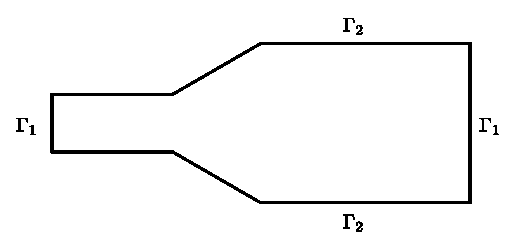
\includegraphics{figure/fig9.3.eps}
\caption{}\label{fig9.3}
\end{figure}

The\pageoriginale potential flow at transonic speed in a nozzle is
governed by the equations
\begin{align*}
&\Div(\rho\overrightarrow{q})=0,\\
&\rot \overrightarrow{q}=0,\overrightarrow{q}=\nabla\phi,\\
&\rho=\left(1-\frac{\gamma-1}{2}M_\infty^2(1-q^2)\right)^{1/\gamma-1}.
\end{align*}
(Practical value of $\gamma=1.4$) where $q=|\overrightarrow{q}|$. 

Finally we solve
$$
\Div(\rho(|\nabla\phi|)\nabla\phi)=0,
$$
\begin{align*}
\phi|_{\Gamma_1} &=\phi_\circ,\\
\frac{\partial\phi}{\partial n}|_{\Gamma_2} &=0
\end{align*}
Let $M=q/a$, where $a=\frac{\rho^{\gamma-1}}{M_\infty^2}$. $M$ is called the
\emph{Mach number}.

The equation is elliptic for $M<1$ and hyperbolic for $M>1$.

When $M<1$ continuous piecewise linear finite element can be used. For
$M>1$, we do not know much (see COURANT- FRIEDRICHS \cite{key13}).

The reader can refer to GLOWINSKI-PIRONNEAU \cite{key20},\cite{key21},\break
RAVIART \cite{key36}, CIAVALDINI-POGU-TOURNEMINE \cite{key12},\break J. ROUX~\cite{key40}.
\end{exam}



\begin{thebibliography}{99}
\addcontentsline{toc}{chapter}{Bibliography}
\bibitem{key1} ADAMS,\pageoriginale R.A.: \emph{Sobolev Spaces},
Academic Press, 1976.

\bibitem{key2} AMARA, M. and J.M. THOMAS: \emph{Une m\'ethode
  d'\'el\'ements finis \'equilibre pour le probl\`eme de
  l'\'elasticit\'e lin\'eaire}, C.R. Acad. Sci. Paris, S\'erie A,
  S\'eance du 3 Avril 1978.

\bibitem{key3} BERCOVIER, M. and O. PIRONNEAU: \emph{Estimations d'erreur
  pour la r\'esolution du probl\`eme de STokes en \'el\'ements finis
  conformes de Lagrange}, C.R. Acad. Sci. Paris, t 285 S\'erie A
  (1977), 557 -- 559.

\bibitem{key4} BR\'EZIS, H.: \emph{Operateurs Maximaux Monotones},
  Lecture Notes \# 5, North Holland, 1975, RAIRO, 1974.

\bibitem{key5} BREZZI, F.: \emph{On the existence, Uniqueness and
  Approximation of Saddle point problems arising from lagrangian
  multipliers}, RAIRO, Vol. 8, 1974, 129 -- 151.

\bibitem{key6} BREZZI, F.; J. RAPPAZ and P.A. RAVIART: \emph{Finite
  element approximation of bifurcation problem (to appear)}.

\bibitem{key7} BREZZI, F. and P.A. RAVIART: \emph{Mixed finite element
  methods for $4^{th}$ order elliptic equations}, Topics in Numerical
  Analysis III, ed. by John, J.H. Miller, Academic Press, 33 -- 57.

\bibitem{key8} BROWDER, F.E. and W.V. PETRYSHN: \emph{Construction of
  fixed points of nonlinear mappings in Hilbert Spaces},
  J. Math. Anal. Appl., 20 (1977), 197 -- 228.

\bibitem{key9} CIARLET,\pageoriginale P.G.: \emph{The Finite Element Method 
for elliptic problems}, North Holland, 1978.

\bibitem{key10} CIARLET, P.G. and P.A. RAVIART: \emph{A Finite Element
  Method for the Biharmonic Equation}, Mathematical Aspects of Finite
  Elements in Partial Differential Equations, by Carl de Boor,
  Academic Press, 1974, 125 -- 146.

\bibitem{key11} CIAVALDINI, J.F. and J.C. NEDELEC: \emph{Sur l'element
  de Fraeijs de Veubeke et Sander}, Serie Analyse Numerique, RAIRO,
  1974, 29 -- 46.

\bibitem{key12} CIAVALDINI, J.F.: M.POGU and G. TOURMINE: \emph{Une
  nouvelle approche daus le plan physique pour le calcul d'elements
  subcritiques et Stationnaires autour d'un profil portant}, Journal
  de m\'ecanique, 16 (1977) 257 -- 288.

\bibitem{key13} COURANT, R and K.O. FRIEDRICHS: \emph{Supersonic flow
  and Shock Waves}, J. Wiley, 1948.

\bibitem{key14} CROUZEIX, M. and P.A. RAVIART: \emph{Conforming and
  Nonconforming Finite Elements Methods for solving the Stationary
  Stokes Equations}, RAIRO, 1974, 1 -- 53.

\bibitem{key15} EKELAND, I. and R. THEMAN: \emph{Convex Analysis and
  Variational Problems}, North-Holland, 1976.

\bibitem{key16} FORTIN, M.: \emph{Approximation des Fonctions a
  Divergence Nulle par la Methode des Elements Fini}, Springer-Verlag
  Lecture Notes in Physics, \# 18, 1972, 99 -- 103.

\bibitem{key17} FORTIN,\pageoriginale M.: \emph{R\'esolution Numerique
  des Equations de Navier-Stokes par des El\'ements Fini de type
  Mixte}, IRIA Report, \# 184, 1976.

\bibitem{key18} FORTIN, M: \emph{Analysis of the convergence of mixed
  finite element methods}, Serie Numerical Analysis, RAIRO, 1977 341
  -- 354.

\bibitem{key19} GLOWINSKI, R. and MARROCCO: \emph{Approximation par
  \'el\'ements Finis d'ordre un et resolution par p\'enalisation
  dualite d'une classe de problemes nonlineari\`es}, Serie Analyse
  Numerique, RAIRO, 1975, 41 -- 76.

\bibitem{key20} GLOWINSKI, R.; J. PERIAUX and O. PIRONNEAU: \emph{Use
  of Optimal Control Theory for the Numerical Simulation of Transonic
  Flow by the Method of Finite Elements}, Springer-Verlag, Lecture
  Notes in Physics, \# 59, 1976, 205 -- 211.

\bibitem{key21} GLOWINSKI, R. and O. PIRONNEAU: \emph{Calcul d
  ecoulements transoniques par des m\'ethodes d'\'el\'ements finis et
  de controle optimal}, Springer-Verlag Lecture Notes in Economics and
  Mathematical systems, \# 134, 1975, 276 -- 296.

\bibitem{key22} GRISVARD, P.: \emph{Behaviour of the solutions of an
  Elliptic Boundary Value Problem in a polygonal or polyhedral Domain},
  Numerical Solution of Partial Differential Equations III, Synspade,
  1975, ed. by Vert Hubbard, Academic Press, 1976, 207 -- 274.

\bibitem{key23} JAMET,\pageoriginale P. and P.A. RAVIART:
  \emph{Numerical solution of the stationary Navier-Stokes Equations
    by finite element methods}, Springer-Verlag Lecture Notes in
  Computer Science, \# 10, 1973, 193 -- 223.

\bibitem{key24} JOHNSON, C: \emph{On the convergence of some mixed
  finite element methods in plate bending problems}, Num. Math. 21
  (1973), 43 -- 62.

\bibitem{key25} JOHNSON, C. and B. MERCIER: \emph{Some mixed finite
  element methods for elasticity problems}, Num. Math., 30 (1978) 103
  -- 116.

\bibitem{key26} KATO, T.: \emph{Perturbation Theory for linear
  operators}, Springer-Verlag 1976.

\bibitem{key27} LADYZHENSKAYA, O.A.: \emph{The Mathematical Theory of
  Viscous Incompressible Flow}, Gorden and Breach, 1969.

\bibitem{key28} LIONS, J.L.: \emph{Quelques m\'ethodes de r\'esolution
  des probl\`ems aux limites nonlin\'earies}, Paris, Dunod, 1969.

\bibitem{key29} LIONS, J.L. and E. MAGENES: \emph{Non Homogeneous
  Boundary Value Problems and Applications}, Vol. I, Springer-Verlag,
  1973.

\bibitem{key30} LUENBERGER, D.G.: \emph{Introduction to linear and
  nonlinear programming}, Addison-Wesley, 1973.

\bibitem{key31} LUENBERGER, D.G.: \emph{Optimization by Vector Space
  Methods}, John Wiley, 1969.

\bibitem{key32} MERCIER, B. and O. PIRONNEAU: \emph{Some Examples of
  implementation and of application of the finite element method},

\bibitem{key33} NE$\check{C}$AS,\pageoriginale J: \emph{Les m\'ethodes
  directes en theorie des equations elliptiques}, Masson, 1967.

\bibitem{key34} OSBORN, J.E.: \emph{Spectral approximation for compact
  operators}, Mathematics of Computations, 29 (1975) 712 -- 725.

\bibitem{key35} PAIGE, C.C. and M.A. SAUNDERS: \emph{Solution of
  sparse indefinite systems equations}, SIAM, J. Num. Analysis, 12
  (1975), 617 -- 629.

\bibitem{key36} RAVIART, P.A.: \emph{Journees elements finis},
  Conference, Rennes, 1978.

\bibitem{key37} RAVIART, P.A. and J.M. THOMAS: \emph{Primal hybrid
  finite element methods for $2^{nd}$ order Elliptic equations},
  Mathematics of Computations, 31 (1977), 391 -- 413.

\bibitem{key38} RAVIART, P.A. and J.M. THOMAS: \emph{A mixed finite
  element method for second order elliptic problems}, Springer-Verlag
  Lecture Notes, \# 606, ed. by Galligani, I. and E. Magenes (1975),
  292 -- 315.

\bibitem{key39} de RHAM, G.: \emph{Varietes differentiables}, Hermann,
  1950.

\bibitem{key40} ROUX, J.: \emph{Resolution Numerique d'un probleme d
  Ecoulement Subsonique de Fluides Compressibles}, Springer-Verlag
  Lecture Notes in Physics, \# 59, 1976, 360 -- 369.

\bibitem{key41} SCHOLZ, R.: \emph{A mixed method for $4^{th}$ order
  problems using linear finite elements}, Serie Numerical Analysis,
  RAIRO, Vol. 12, 1978, 85 -- 90.

\bibitem{key42} TAYLOR,\pageoriginale C. and P. HOOD: \emph{A
  numerical solution of the Navier-Stokes Equation using the finite
  elements technique}, Computers and Fluids, Vol. I, 1973, 73 -- 100.

\bibitem{key43} TEMAN, R.: \emph{On the theory and numerical analysis
  of Navier-Stokes equations}, North-Holland, 1977.

\bibitem{key44} THOMEE, V. : \emph{Some convergence results for
  Galerkin Methods for Parabolic Boundary Value Problems},
  Mathematical Aspects of Finite Elements in Partial Differential
  Equations, ed. by Carl de Boor, Academic Press, 1974, 55 -- 88.

\bibitem{key45} THOMEE, V.: \emph{Some Error Estimates in Galerkin
  Methods for Parabolic Equations}, Springer-Verlag Lecture Notes in
  Mathematics, \# 606, 1975, 343 -- 352.

\bibitem{key46} YOSIDA, K.: \emph{Functional Analysis},
  Springer-Verlag, 1974.

\bibitem{key47} SIENKIEWICZ, O.C.: \emph{Why Finite Elements\@?}
  Finite elements in Fluids, Vol. I, ed. by Gallagher, John Wiley,
  1975, 1 -- 24.
\end{thebibliography}



